\documentclass[a4paper,12pt]{article}
\usepackage[top = 2.5cm, bottom = 2.5cm, left = 2.5cm, right = 2.5cm]{geometry}
\usepackage[T1]{fontenc}
\usepackage[utf8]{inputenc}
\usepackage{multirow} 
\usepackage{booktabs} 
\usepackage{graphicx}
\usepackage[spanish]{babel}
\usepackage{setspace}
\setlength{\parindent}{0in}
\usepackage{float}
\usepackage{fancyhdr}
\usepackage{amsmath}
\usepackage{amssymb}
\usepackage{amsthm}
\usepackage{natbib}
\usepackage{graphicx}
\usepackage{subcaption}
\usepackage{booktabs}
\usepackage{etoolbox}
\usepackage{apalike}
\usepackage{minibox}
\usepackage{hyperref}
\usepackage{xcolor}
\usepackage{tcolorbox}
\newcommand{\linea}{\noindent\rule{\textwidth}{1pt}}
\AtBeginEnvironment{align}{\setcounter{equation}{0}}
\newenvironment{solution}
  {\renewcommand\qedsymbol{$\square$}\begin{proof}[\textcolor{blue}{Solución}]}
  {\end{proof}}

\pagestyle{fancy}

\fancyhf{}

\lhead{\footnotesize Estadística Matemática}
\rhead{\footnotesize  Rudik Roberto Rompich}
\cfoot{\footnotesize \thepage}

\begin{document}
    \thispagestyle{empty} 
    \begin{tabular}{p{15.5cm}}
    \begin{tabbing}
    \textbf{Universidad del Valle de Guatemala} \\
    Departamento de Matemática\\
    Licenciatura en Matemática Aplicada\\\\
   \textbf{Estudiante:} Rudik Roberto Rompich\\
   \textbf{E-mail:} \textcolor{blue}{ \href{mailto:rom19857@uvg.edu.gt}{rom19857@uvg.edu.gt}}\\
   \textbf{Carné:} 19857
    \end{tabbing}
    \begin{center}
        MM2036 - Estadística Matemática - Catedrático: Paulo Mejía\\
        \today
    \end{center}\\
    \hline
    \\
    \end{tabular} 
    \vspace*{0.3cm} 
    \begin{center} 
    {\Large \bf Parcial 4
} 
        \vspace{2mm}
    \end{center}
    \vspace{0.4cm}
%---------------------------
%\begin{tcolorbox}[colback=gray!15,colframe=black!1!black,title=A nice heading]
%\end{tcolorbox}

%\fbox{lol}
%---------------------------


%-----------------------------
Instrucciones: Resuelva los siguientes problema. Favor hacer la solución en latex y cargar el archivo latex y pdf en la tarea de Canvas. Para la resolución de los problemas, se utilizará el libro de \cite{wackerly2014mathematical}. 
\section{Problema 1}


Sea $Y_{1}, Y_{2}, \ldots, Y_{n}$ una muestra aleatoria de una distribución normal con media $\mu$ y varianza $1 .$
\begin{tcolorbox}[colback=gray!15,colframe=black!1!black,title=Definición 4.8 - Distribución Normal]
	A random variable $Y$ is said to have a normal probability distribution if and only if, for $\sigma >0$ and $-\infty<\mu<\infty$, the density function of $Y$ is
	$$f(y)=\frac{1}{\sigma\sqrt{2\pi}}e^{-(y-\mu)^2/(2\sigma^2)}, \qquad \infty<y<\infty$$
	\end{tcolorbox}
\begin{enumerate}
	\item a) Demuestre que $\overline{Y}$ es un estimador suficiente para $\mu$.
	\begin{solution}
		Comenzamos definiendo al estimador suficiente como:
		\begin{tcolorbox}[colback=gray!15,colframe=black!1!black,title=Teorema 9.4 - Estimador suficiente]
			Let $U$ be a statistic based on the random sample $Y_1, Y_2,..., Y_n$. Then $U$ is a sufficient statistic for the estimation of a parameter $\theta$ if and only if the likelihood $L(\theta) = L(y_1, y_2, . . . , y_n | \theta)$ can be factored into two nonnegative functions,
			$$L(y_1,y_2,...,y_n |\theta)=g(u,\theta)\times h(y_1, y_2,..., y_n)$$
			where $g(u,\theta)$ is a function only of $u$ and $\theta$ and $h(y_1,y_2,...,y_n)$ is not a function of $\theta$.
		\end{tcolorbox}
	\begin{align*}
		L(y_1,y_2,\cdots, y_n|\mu) &= L(y_1|\mu)\times L(y_2|\mu)\times \cdots \times L(y_n|\mu)\\
		&=
			\frac{1}{\sigma\sqrt{2\pi}}\exp\left[{-(y_1-\mu)^2 \over (2\sigma^2)}\right]\times \frac{1}{\sigma\sqrt{2\pi}}\exp\left[{-(y_2-\mu)^2 \over (2\sigma^2)}\right]\times \cdots \times\\
			& \times \cdots \times\frac{1}{\sigma\sqrt{2\pi}}\exp\left[{-(y_n-\mu)^2 \over (2\sigma^2)}\right]\\
			&= \frac{1}{\sigma^n\left(\sqrt{2\pi}\right)^n}\times \exp\left[-\frac{1}{2\sigma^2}\left(\sum_{i=1}^{n}(y_i-\mu)^2\right)\right]\\
			&= \frac{1}{\sigma^n\left(\sqrt{2\pi}\right)^n}\times \exp\left[-\frac{1}{2\sigma^2}\sum_{i=1}^{n}\left(y^2_i-2y_i\mu+\mu^2\right)\right]\\
			&= \frac{1}{\sigma^n\left(\sqrt{2\pi}\right)^n}\times \exp\left[-\frac{1}{2\sigma^2}\left(\sum_{i=1}^{n}y^2_i-2\sum_{i=1}^{n}y_i\mu+\sum_{i=1}^{n}\mu^2\right)\right]\\
			&= \frac{1}{\sigma^n\left(\sqrt{2\pi}\right)^n}\times \exp\left[-\frac{1}{2\sigma^2}\left(\sum_{i=1}^{n}y^2_i-2n\overline{y}\mu+n\mu^2\right)\right]
			\intertext{Se conocía que $\sigma^2$=1, por lo cual:}
			&= \frac{1}{\left(\sqrt{2\pi}\right)^n}\times \exp\left[-\frac{1}{2}\left(\sum_{i=1}^{n}y^2_i-2n\overline{y}\mu+n\mu^2\right)\right]\\
			&= \frac{1}{\left(\sqrt{2\pi}\right)^n}\times \exp\left[-\frac{1}{2}\sum_{i=1}^{n}y^2_i+\frac{1}{2}2n\overline{y}\mu-\frac{1}{2}n\mu^2\right]\\
			&= \left\{\frac{1}{\left(\sqrt{2\pi}\right)^n}\times \exp\left[-\frac{1}{2}\sum_{i=1}^{n}y^2_i\right]\right\}\times\exp\left[n\overline{y}\mu-\frac{1}{2}n\mu^2\right]\\
			&= h(y)\times g(\overline{y},\mu)
			\end{align*}
		Por lo tanto, $\overline{y}$ es un estimador suficiente para $\mu$.
	\end{solution}
	\item b) ¿Cuál es la distribución de $\overline{Y}$ con sus parámetros? (Incluya la justificación).
	\begin{solution}
		Considérese el teorema 4.7:
		\begin{tcolorbox}[colback=gray!15,colframe=black!1!black,title=Teorema 7.1 ]
			Let $Y_1, Y_2, . . . , Y_n$ be a random sample of size n from a normal distribution 
			with mean $\mu$ and variance $\sigma$. Then
			$$\overline{Y}=\frac{1}{n}\sum_{i=1}^{n}Y_i$$
			is normally distributed with mean $\mu_{\overline{Y}} = \mu$ and variance $\sigma^2_{\overline{Y}} = \sigma^2/n$.
		\end{tcolorbox}
Entonces, podemos concluir que $\overline{Y}$ tiene una distribución normal con media $\mu_{\overline{Y}} = \mu$ y varianza $\sigma^2_{\overline{Y}} = 1/n$.
	\end{solution}
	\item c) Encuentre la función generadora de momentos de $\overline{Y}$ (Incluya la justificación).
	\begin{solution}
		Vamos a tomar como referencia el cuadro 2 del apéndice 2: 
		\begin{center}
			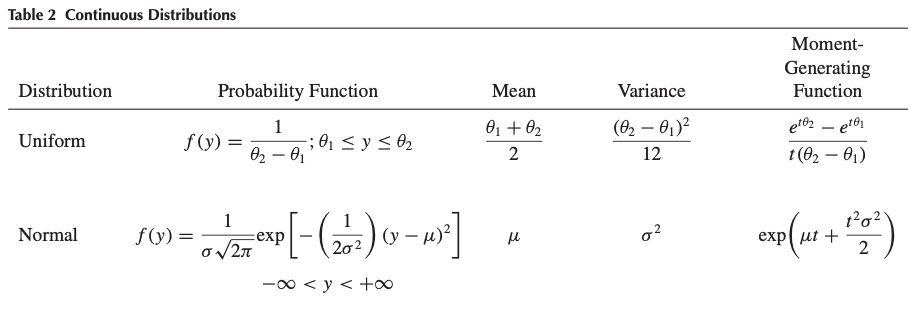
\includegraphics[scale=0.4]{/Users/rudiks/Git/Estadistica_Matematica/Parcial4/Images/Screen Shot 2021-05-23 at 20.39.19.png}
		\end{center}
	La demostración del caso general es la siguiente: 
	\begin{align*}
		m_U(t) &= E(\exp(tU))\\
					   &= \int_{-\infty}^{\infty} \exp(tU)\cdot f(U)dU\\
		      		   &=\frac{1}{\sigma \sqrt{2 \pi}} \int_{-\infty}^{\infty} \exp \left(t U-\frac{(U-\mu)^{2}}{2 \sigma^{2}}\right) \mathrm{d} U \\
						&=\frac{\sqrt{2} \sigma}{\sigma \sqrt{2 \pi}} \int_{-\infty}^{\infty} \exp \left((\sqrt{2} \sigma z+\mu) t-z^{2}\right) \mathrm{d} z \quad \text { sustituyendo } z=\frac{U-\mu}{\sqrt{2} \sigma} \\
				   		&=\frac{\exp\{\mu t\}}{\sqrt{\pi}} \int_{-\infty}^{\infty} \exp \left(-\left(z^{2}-\sqrt{2} \sigma z t\right)\right) \mathrm{d} z \\
				   		&=\frac{\exp\{\mu t\}}{\sqrt{\pi}} \int_{-\infty}^{\infty} \exp \left(-\left(z-\frac{\sqrt{2}}{2} \sigma t\right)^{2}+\frac{1}{2} \sigma^{2} t^{2}\right) \mathrm{d} z \\
				   		&=\frac{\exp \left(\mu t+\frac{1}{2} \sigma^{2} t^{2}\right)}{\sqrt{\pi}} \int_{-\infty}^{\infty} \exp \left(-v^{2}\right) \mathrm{d} v \quad \text { sustituyendo } v=z-\frac{\sqrt{2}}{2} \sigma t \\
				   		&=\frac{\sqrt{\pi} \exp \left(\mu t+\frac{1}{2} \sigma^{2} t^{2}\right)}{\sqrt{\pi}} \quad \\
				       &=\exp \left(\mu t+\frac{1}{2} \sigma^{2} t^{2}\right)
				       \intertext{Para el caso en donde $\sigma^2=1$}
				       &=\exp \left(\mu t+\frac{1}{2}  t^{2}\right)
	\end{align*}
	\end{solution}
	\item d) Calcule $E\left(\overline{Y}^{2}\right)$ y $E\left(\overline{Y}^{4}\right)$, utilizando la función generadora de momentos del inciso de
	$\overline{Y}$.
	\begin{solution}
		Según la literatura:
		\begin{tcolorbox}[colback=gray!15,colframe=black!1!black,title=Valor esperado]
			$$E(Y^n)=M^{(n)}_Y(0)=\frac{d^nM_Y(0)}{dt^n}$$
			\end{tcolorbox}
		Entonces: 
		\begin{center}
			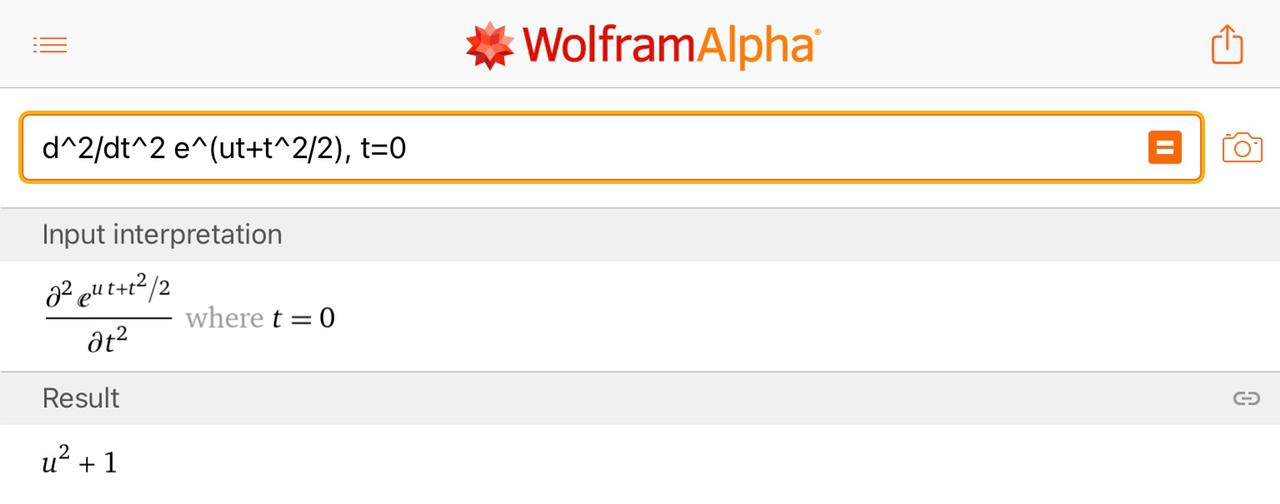
\includegraphics[scale=0.3]{/Users/rudiks/Git/Estadistica_Matematica/Parcial4/Images/WhatsApp Image 2021-05-23 at 21.48.55.jpeg}
		\end{center}
		$$E(Y^2)=M^{(2)}_Y(0)=\frac{d^2M_Y(0)}{dt^2}=\mu^2+1$$
		Entonces, tenemos $E(Y^2_i)=\mu^2+1$ por la deducción del teorema 5.12, podemos asumir que: 
		$$E(\overline{Y}^2)=\mu^2+\frac{1}{n}.$$
		Por otra parte,
		\begin{center}
			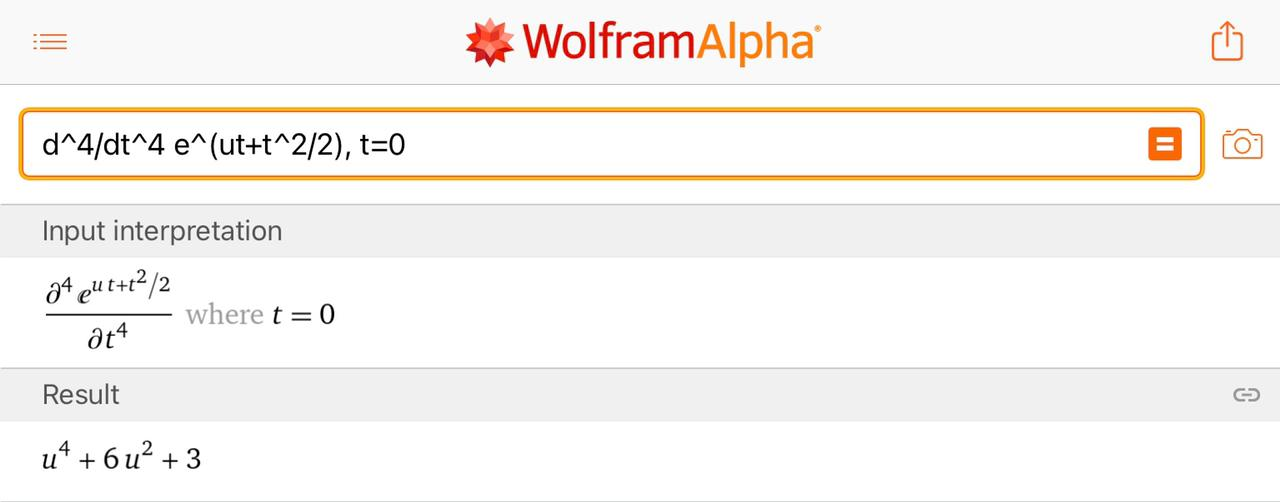
\includegraphics[scale=0.3]{/Users/rudiks/Git/Estadistica_Matematica/Parcial4/Images/WhatsApp Image 2021-05-23 at 21.48.55-2.jpeg}
		\end{center}
		$$E(Y^4)=M^{(4)}_Y(0)=\frac{d^4M_Y(0)}{dt^4}=\mu^4+6\mu^2+3$$
		Entonces, tenemos $E(Y^4_i)=\mu^4+6\mu^2+3$ por la deducción del teorema 5.12, podemos asumir que: 
		$$E(\overline{Y}^4)=\mu^4+\frac{6\mu^2}{n}+\frac{3}{n^2}.$$
	\end{solution}
    \item e) Demuestre que el MUEV (estimador insesgado de varianza mínima) de $\mu^{2}$ es $\widehat{\mu^{2}}=$ $\overline{Y}^{2}-\frac{1}{n}$. \begin{solution}
    	Sabemos que $\overline{Y}$ es suficiente para $\mu$. Además, sabemos que $\sigma$=1, por lo que $\overline{Y}$ tiene una distribución normal con media $\mu$ y varianza $1/n$.  Entonces,
    	
    	$$E(\overline{Y}^2)=\mu^2 +\frac{1}{n}\implies E\left(\overline{Y}^2-\frac{1}{n}\right)=\mu^2$$  
    	
    	
    	 Entonces, tenemos un estimador insesgado de $\mu^2$. Ahora, tomando en cuenta el siguiente teorema:	\begin{tcolorbox}[colback=gray!15,colframe=black!1!black,title=The Rao–Blackwell Theorem]
    		Let $\hat{\theta}$ be an unbiased estimator for $\theta$ such that
    		$VAR(\hat{\theta}) < \infty$. If $U$ is a sufficient statistic for $\theta$, define $\hat{\theta}^*$ = $E(\hat{\theta} |U)$. Then, for
    		all $\theta$,
    		$$E(\hat{\theta}^*)=\theta \quad \text{ y } \quad VAR(\hat{\theta}^*)\leq VAR(\hat{\theta}).$$
    		\end{tcolorbox}
    	Implica que $\hat{\mu}^2=\overline{Y}^2-\frac{1}{n}$ es un MVUE de $\mu^2$. 
    \end{solution}
	\item f) Obtenga la $V A R\left(\widehat{\mu^{2}}\right)$, utilizando el resultado en $\mathrm{d}$ ).
	\begin{solution}
		$$VAR(\hat{\mu}^2)=VAR\left(\overline{Y}^2-\frac{1}{n}\right)=VAR\left(\overline{Y}^2\right)=E(\overline{Y}^4)-[E(\overline{Y}^2)]^2=$$
		$$=\mu^4+\frac{6\mu^2}{n}+\frac{3}{n^2}-\left[\mu^2+\frac{1}{n}\right]^2=\frac{\left(2+4n\mu^2\right)}{n^2}.$$
	\end{solution} 
\end{enumerate}
(Valor 25 puntos).


\section{Problema 2}


Los estimadores de máxima verosimilitud tienen propiedades interesantes cuando se trabaja con muestras grandes. Suponga que $t(\theta)$ es una función derivable en $\theta$. Por la propiedad de invarianza, se tiene que si $\hat{\theta}$ es el MLE de $\theta$, entonces el MLE de $t(\theta)$ está dada por $t(\hat{\theta}) .$ En algunas condiciones de regularidad que se cumplen para las distribuciones que se consideren, $t(\hat{\theta})$ es un estimador consistente para $t(\theta) .$ Además, para tamaño de muestras grandes,
$$
Z=\frac{t(\hat{\theta})-t(\theta)}{\sqrt{\left[\frac{\partial t(\theta)}{\partial \theta}\right]^{2} \Big/ n E\left[-\frac{\partial^{2} \ln [f(Y \mid \theta)]}{\partial \theta^{2}}\right]}}
$$
tiene aproximandamente una distribución normal estándar, donde $f(Y \mid \theta)$ es la función densidad correspondiente a la distribución continua de interés, evaluada en el valor aleatorio Y. En el caso discreto, el resultado análogo se cumple con la función de probabilidad evaluada en el valor aleatorio $\mathrm{Y}$, $p(Y \mid \theta)$, se sustituye por la densidad $f(Y \mid \theta)$. En el caso particular, para una variable aleatoria con distribución de Bernoulli, $p(y \mid p)=$ $p^{y}(1-p)^{1-y}$, donde $\mathrm{y}=0,1 .$ Si $Y_{1}, \ldots, Y_{n}$ es una muestra aleatoria de tamaño $\mathrm{n}$ de dicha distribución.

\begin{enumerate}
	\item a) Encuentre el MLE para el parámetro p.
	\begin{solution}
		content...
	\end{solution}
	\item b) Encuentre el MLE para la expresión p(1-p).
	\item c) Construya un intervalo de confianza de $100(1-\alpha) \%$ para $\mathrm{p}(1-\mathrm{p})$, la varianza de dicha distribución (suponga una muestra grande).
\end{enumerate}
 (Valor 25 puntos).

\section{Problema 3}

Suponga que $Y_{1}, Y_{2}, \ldots, Y_{n}$ es una muestra aleatoria de la distribución de Poisson con media $\lambda>0$.

\begin{enumerate}
	\item a) Encuentre el estimador del método de momentos para $\lambda$.
	\item b) Encuentre el estimador de máxima verosimilitud (MLE) $\hat{\lambda}$ para $\lambda$. (Valor 25 puntos).
\end{enumerate}

\section{Problema 4}

Sea $Y$ una variable aleatoria que representa el número de éxitos en $\mathrm{n}$ intentos independientes con probabilidad p de éxito en cada intento. Además,
$$
Y=\sum_{i=1}^{n} Y_{i}
$$
donde
$$
Y_{i}=\begin{cases}
	1  , & \text { si el i-ésimo intento resulta en éxito } \\
	0  , & \text { en el otro caso }
\end{cases}
$$
para $\mathrm{i}=1, \ldots, \mathrm{n}$
\begin{enumerate}
	\item a) Demuestre que $\widehat{p_{n}}=\frac{Y}{n}$ es un estimador insesgado de $p$.
	\begin{solution} Tenemos las siguientes denificiones:: 
		\begin{tcolorbox}[colback=gray!15,colframe=black!1!black,title=Definición 8.2 - Sesgo ]
			Let $\hat{\theta}$ be a point estimator for a parameter $\theta$. Then $\hat{\theta}$  is an unbiased estimator if $E(\hat{\theta})=\theta$. If$E(\hat{\theta})\neq \theta$, $\theta$ is said to be biased.
			\end{tcolorbox}
		
		\begin{tcolorbox}[colback=gray!15,colframe=black!1!black,title=Definición 8.3 - Sesgo ]
			The bias of a point estimator $\hat{\theta}$ is given by $B(\hat{\theta}) = E(\hat{\theta}) - \theta $.
		\end{tcolorbox}
	A probar: $E(\hat{p}_n)=p$.  Entonces:

	$$E(\hat{p}_n)=E\left(\frac{Y}{n}\right)=\underbrace{\frac{1}{n}E(Y)}_{\text{Teorema 5.7}}=\frac{1}{n}E\left(\sum_{i=1}^{n}Y_i\right)=\frac{1}{n}E\left(Y_1+Y_2+\cdots +Y_n\right)=$$
	$$=\frac{1}{n}\left[\underbrace{E(Y_1)+E(Y_2)+\cdots + E(Y_n)}_{E(Y_i)=p \text{, definición de valor esperado.}}\right]=\frac{1}{n}\left[p+p+\cdots+p\right]=\frac{1}{n}(np)=p$$
	
	\end{solution}
	\item b) Demuestre que $\widehat{p_{n}}$ es un estimador consistente de $p$.
	\begin{solution} 
		Procedemos a calcular la varianza del estimador, es decir: 
		$$VAR(\hat{p}_n)=\frac{pq}{n}. \quad \text{ (Deducción en el ejercicio 5.28).}$$
		$\implies$ Tomamos como referencia el teorema 9.1:
		\begin{tcolorbox}[colback=gray!15,colframe=black!1!black,title=Teorema 9.1]
			An unbiased estimator $\hat{\theta}_n$ for $\theta$ is a consistent estimator of $\theta$ if
			$$\lim_{n\to\infty}VAR(\hat{\theta}_n)=0.$$
		\end{tcolorbox}
	$$\implies \lim_{n\to\infty}VAR(\hat{p}_n)=\lim_{n\to\infty}VAR\left(\frac{pq}{n}\right)=VAR\left(\frac{pq}{0}\right)=0.$$
	\end{solution}
	\item c) Cuando $\mathrm{n}$ es grande, demuestre que la distribución de $\frac{\widehat{p_{n}}-p}{\sqrt{p(1-p) / n}}$ converge a una distribución normal estándar.
	\begin{solution}
		Considerando: \begin{tcolorbox}[colback=gray!15,colframe=black!1!black,title=Teorema 9.3]
			Suppose that $U_n$ has a distribution function that converges to a standard normal distribution function as $n \to \infty$. If $W_n$ converges in probability to 1, then the distribution function of $U_n / W_n $converges to a standard normal distribution function.
			\end{tcolorbox}
	\end{solution}
	\item d) Cuando $\mathrm{n}$ es grande, demuestre que la distribución de $\frac{\widehat{p_{n}}-p}{\sqrt{p_{n}\left(1-\widehat{p_{n}}\right) / n}}$ converge a una distribución normal estándar. 
	\begin{solution}
		Considerando: \begin{tcolorbox}[colback=gray!15,colframe=black!1!black,title=Teorema 9.3]
			Suppose that $U_n$ has a distribution function that converges to a standard normal distribution function as $n \to \infty$. If $W_n$ converges in probability to 1, then the distribution function of $U_n / W_n $converges to a standard normal distribution function.
		\end{tcolorbox}
	\end{solution}
\end{enumerate}
(Valor 25 puntos)

%---------------------------
\bibliographystyle{apalike}
\bibliography{sample.bib}

\end{document}